%% ==============================
\chapter{\iflanguage{ngerman}{Einleitung}{Introduction}}
\label{sec:Introduction}
%% ==============================

\subsection{Motivation}

Computergestützte Verfahren werden in der Medizin immer wichtiger. Sie erleichtern dem Arzt seine Arbeit und senken die Wahrscheinlichkeit, dass bei einer Operation ein Fehler gemacht wird.
\newline
Ein Routineprozedur der Neurochirurgie ist die Punktion des Ventrikelsystems zur Drainage von Liquor. Diese wird häufig nötig, wenn ein Patient beispielsweise unter einer Gehirnblutung, einem Schädelhirntrauma oder einem Schlaganfall leidet.
\newline
Um die Punktion durchzuführen, muss der Chirurg eine Bohrlochtrepanation am sogenannten Kocherpunkt durchführen. Der Arzt muss dabei anhand äußerer anatomischer Landmarker diesen Punkt auf wenige Zentimeter genau finden und die Stichrichtung der Punktion ausmachen.



\subsection{Problemstellung}

Das aktuelle Vorgehen bei einer Ventrikelpunktion ist sehr fehleranfällig. So kommt es nur in zwei drittel aller Operationen zu einem optimalen Ergebnis, wofür oftmals mehrfach punktiert werden muss. In \autoref{fig:punktion} ist ein Bild eines solchen Eingriffs zu sehen. Es ist zu erkennen wie der Chirurg mit dem linken Zeigefinger den inneren Augenwinkel zur Orientierung abtastet, um die Punktion im richtigen Winkel auszuführen.


\begin{figure}[!h] 
\centering 
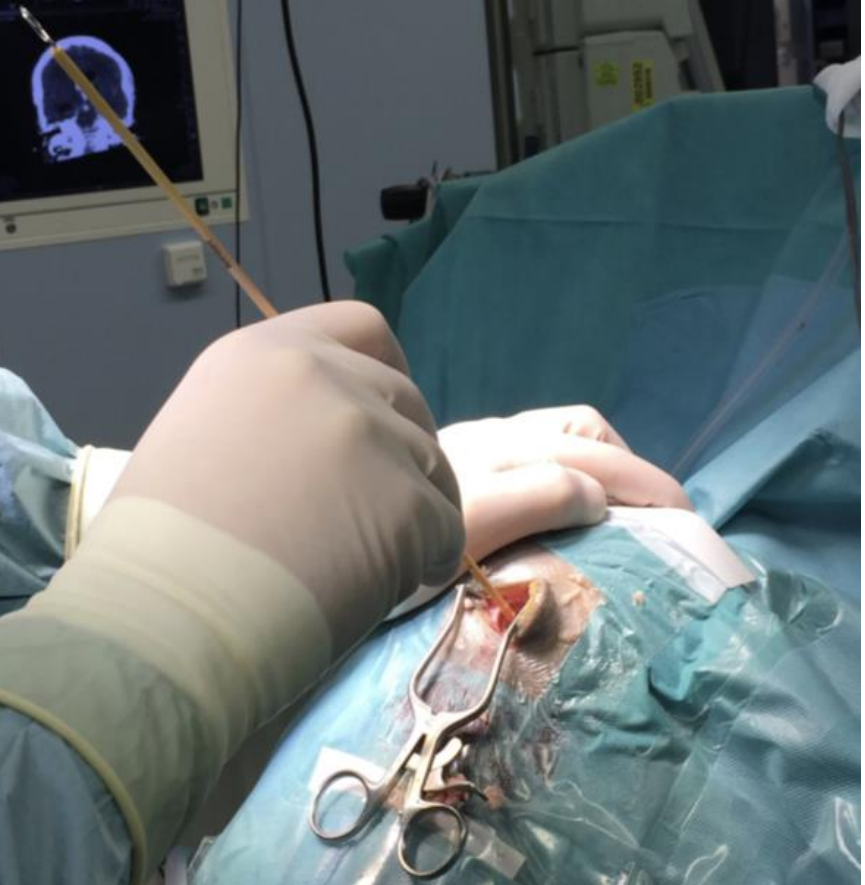
\includegraphics[width=0.6\textwidth]{Logos/Punktion2.png}
\caption{Fotografie einer Ventrikelpunktion  \\ Entnommen aus dem Forschungsprojekt HoloMed \protect\cite{punktion}} 
\label{fig:punktion} 
\end{figure}


Im Rahmen des HoloMed Projektes wird daran gearbeitet den Chirurg bei diesem Eingriff zu unterstützen. Der Plan ist es, dass der Arzt mithilfe einer AR-Brille angezeigt bekommt wo sich das Ventrikelsystem befindet und somit mit einer niedrigeren Fehlerwahrscheinlichkeit die Operation durchführen kann. Daraus ergibt sich die Aufgabe das Ventrikelsystem anhand von CT-Daten des Gehirns zu segmentieren und hervorzuheben.



\subsection{Zielsetzung}

Zum Lösen dieser Problemstellung eignen sich Übergangsfunktionen, auch Transferfunktionen genannt. Allgemein gesprochen ordnet eine Transferfunktion volumetrischen Daten optische Eigenschaften zu. Diese Aufgabe teilt sich in zwei Bereiche auf. Zum einen muss die Funktion entscheiden, welche Daten gezeigt werden und zum anderen, wie diese hervorgehoben werden, beispielsweise welche Farb- und Okklusionswerte diese erhalten sollen. Dabei ist der erste Teil der deutlich wichtigere und schwieriger umzusetzende.
\newline
Das Ziel dieser Bachelorarbeit ist es, eine geeigneten Transferfunktion zu Implementieren, um das Ventrikelsystem in CT-Daten segmentieren und hervorheben zu können.



\subsection{Aufbau der Arbeit}

Der Rest dieser Arbeit teilt sich folgendermaßen auf. In Kapitel 2, \nameref{sec:state_of_the_art}, wird ein Überblick über existierenden Transferfunktionen und deren Funktionsweisen gegeben, während sich Kapitel 3, \nameref{sec:methods}, mit der in dieser Arbeit verwendeten Transferfunktion beschäftigt. In Kapitel 4, \nameref{sec:concept}, wird das Softwaredesign der Implementierung erklärt und in Kapitel 5, \nameref{sec:implementation}, die Umsetzung dessen besprochen. Weiterhin wird in Kapitel 6, \nameref{sec:results}, die Resultate dieser Arbeit gezeigt und evaluiert. In Kapitel 7, \nameref{sec:discussion}, wird ein Fazit gezogen und Kapitel 8, \nameref{sec:conclusion}, zeigt mögliche Verbesserungen auf.